\documentclass[pdf]{beamer}
\ProvidesPackage{preamble_slides}

% %% Beamer Stuff
\usetheme{Berlin}
\setbeamertemplate{footline}[frame number]
\setbeamertemplate{caption}[numbered]
\setbeamertemplate{section in toc}[sections numbered]
\setbeamertemplate{subsection in toc}[sections numbered]
\setbeamertemplate{navigation symbols}{} 
\setbeamercovered{transparent=25}
\usepackage{graphicx}
\usepackage{hhline}
\usepackage{appendixnumberbeamer}
\usepackage{multirow}
\definecolor{maincolor}{rgb}{0.6, 0.4, 0.7}
\usecolortheme[named = maincolor]{structure}
\renewcommand{\arraystretch}{1.5}

%% Bibliography packages
\usepackage{natbib}
\bibliographystyle{abbrvnat}

\title{Chinese Head Tax Project: Updates}
\author{Amy Kim}
\date{September 6, 2023}

\begin{document}
\begin{frame}[plain]
    \titlepage
\end{frame}

\begin{frame}{Research Question}
    How does an increase in fixed migration costs (in the form of a nationality-specific flat `head tax' at the time of entry) affect selection into immigration?
\end{frame}
\section{New Data?!}
\begin{frame}
    \frametitle{New Data?! HK Harbormaster Reports}
    \begin{itemize}
        \item Extremely detailed records of each 'passenger' ship (1870-1895) to depart \textbf{and} arrive in Hong Kong -- name, of ship, number of passengers, destination port(s) 
        \item Starting in 1895, still have aggregated number of emigrants/immigrants departing to/arriving from each port 
        \item All years are scanned, but data doesn't seem to be digitized anywhere :( 
    \end{itemize}
\end{frame}

\begin{frame}[label = departure]
    \frametitle{Departure Records}
    \begin{itemize}
        \item Counts number of passengers on ``Chinese Passenger Ships cleared by the emigration officer, Hong Kong" \hyperlink{hk_departure}{\beamerbutton{1895 Departures Record}}
        \item Potential issues: 
        \begin{enumerate}
            \item Might include non-Chinese outbound passengers? (Likely minimal -- crew counted separately, table specifies emigration)
            \item How to consider `transfers', i.e. passengers travelling to different destination via Canada, or to Canada via US
            \item How much of emigration to Canada was out of Hong Kong?
        \end{enumerate}
        \item Answer to (3): likely most -- out of 1,831 registrations in 1895, I can match 1,632 to ships departing from HK. Essentially all other registrations came from US \hyperlink{reg_summ}{\beamerbutton{1895 Matching Example}} (But would need to verify for other years)
    \end{itemize}
\end{frame}

\begin{frame}[label = return]
    \frametitle{Return Records}
    \begin{itemize}
        \item Counts number of passengers on ``Vessels bringing Chinese Passengers to the Port of Victoria, Hong Kong, from Places out of the Chinese Empire" \hyperlink{hk_return}{\beamerbutton{1895 Returns Record}}
        \item Potential issues: 
        \begin{enumerate}
            \item How much of passenger traffic was into Port of Victoria (ans: approx 99.9\% in 1895)
            \item Does this include non-immigrants like merchants, temporary travellers? (ans: seems like no -- table described as reporting passengers ``...brought to Hong Kong from places to which they had emigrated'')
            \item `Transfer' issue likely less problematic -- no reason to return from less convenient place, since easy to leave North America 
            \item How much of return immigration from Canada was into Hong Kong? (ans: again, less of a problem than for emigration -- McKeown (2010): ``Migration data, however, suggest that migrants were much more likely to return via Hong Kong than to depart this way.'')
        \end{enumerate}
    \end{itemize}
\end{frame}

\begin{frame}
    \frametitle{1895 Accounting Exercise}
    \begin{itemize}
        \item 3,714 departures from Hong Kong to Canada 
        \item 1,831 registrations in Canada (49\%)
        \item 2,353 returns (470 `excess' returns beyond `rejections')
    \end{itemize}
    I can also do this with individual ships! E.g. the Empress of China departed HK on 1/23/1895 with 71 passengers. On 2/13/1895, 41 Chinese immigrants were recorded in the Register as having arrived on the Empress of China (implies 30 were rejected, or otherwise never recorded?). Can I proxy rejections like this? On 3/28/1895, the Empress of China returned to HK with 65 passengers. Can I proxy return migrants like this (65 - 30)? 
\end{frame}

\begin{frame}
    \frametitle{Goals with this Data}
    \begin{itemize}
        \item Digitize summary tables (total emigration to Canada, total return migration from Canada by year)
        \item Use number of emigrants out of HK as a separate outcome variable for Time Series regressions (in addition to number of immigrants into CA)
        \item Use number of return migrants into HK as separate outcome variable
        \item Would having individual ship records be helpful? Accounting exercise seems more illustrative as an example than useful as a finding.
    \end{itemize}
\end{frame}

\section{Misc. History}
\begin{frame}[label = chinaflow]
    \frametitle{Emigration from China: Larger Context}
    \begin{itemize}
        \item ~90\% of emigration from China between 1840 and 1940 was to SE Asia (even higher after the 1880s)
        \item So even pre-regulation, Chinese immigrants to North America were a selected group (selected on what?)
        \item Tiny dips in overall/SE Asia emigration in Head Tax years -- concerning?  \hyperlink{china_emig_mckeown}{\beamerbutton{South China Emigration (McKeown 2010)}}
    \end{itemize}
\end{frame}

\begin{frame}[label = immflow]
    \frametitle{Immigration to Canada}
    \centering
    \begin{figure}
        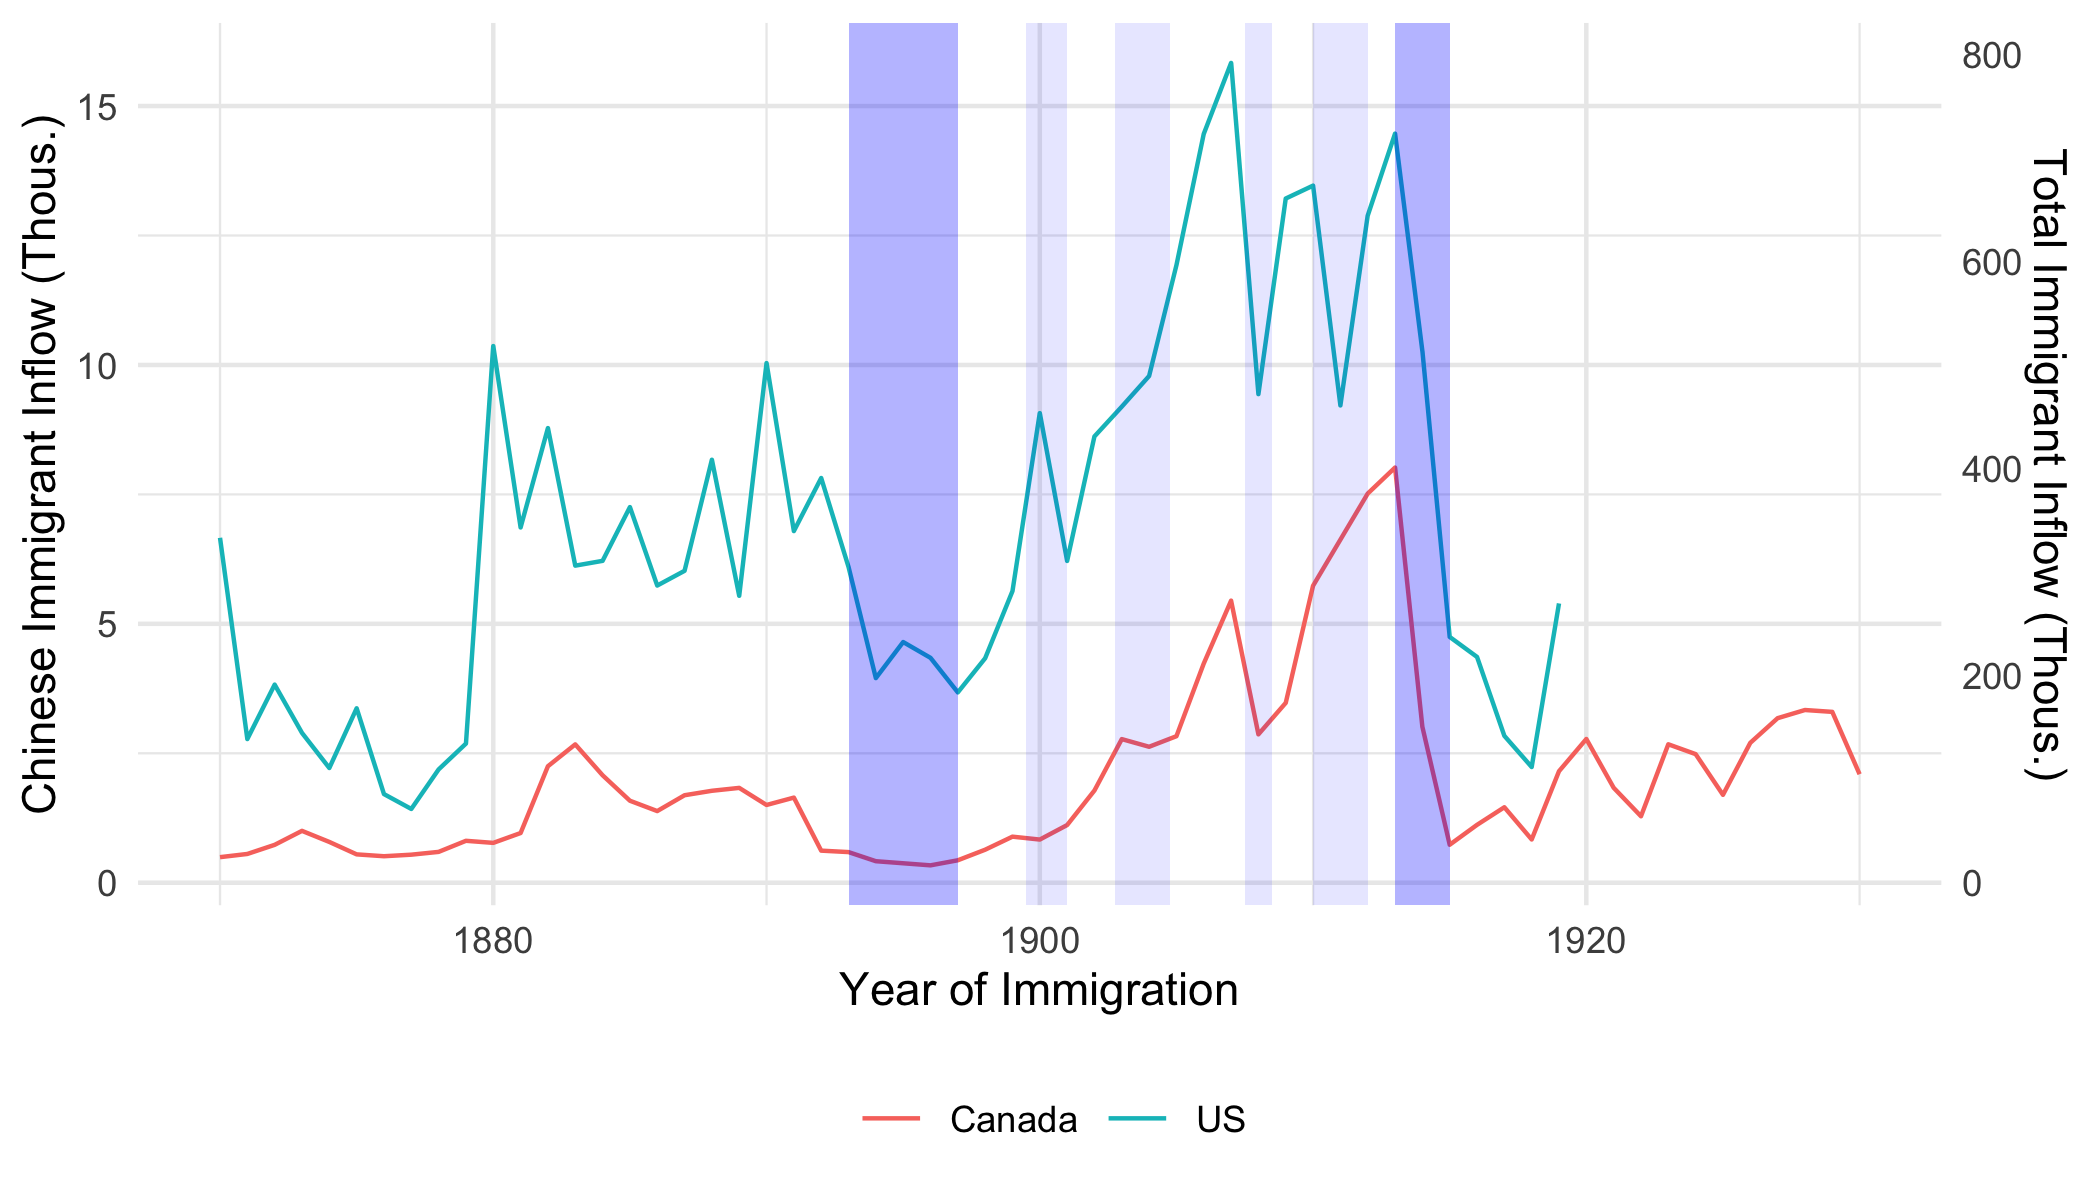
\includegraphics[width = \textwidth]{../../figs/6sep23/immflow.png}
    \end{figure}
\end{frame}

\begin{frame}
    \frametitle{Explaining the 1896-1913 Immigration Boom}
    \begin{itemize}
        \item Coats, in Willcox (1931), explains this boom with a huge amount of foreign investment from Great Britain, ostensibly to fund agricultural production for its empire
        \item Basically identical to US pattern, except missing drops for some of the recessions
    \end{itemize}
\end{frame}

\begin{frame}[label = japan_flow]
    \frametitle{Japanese Migration to Canada}
    \centering
    \begin{figure}
        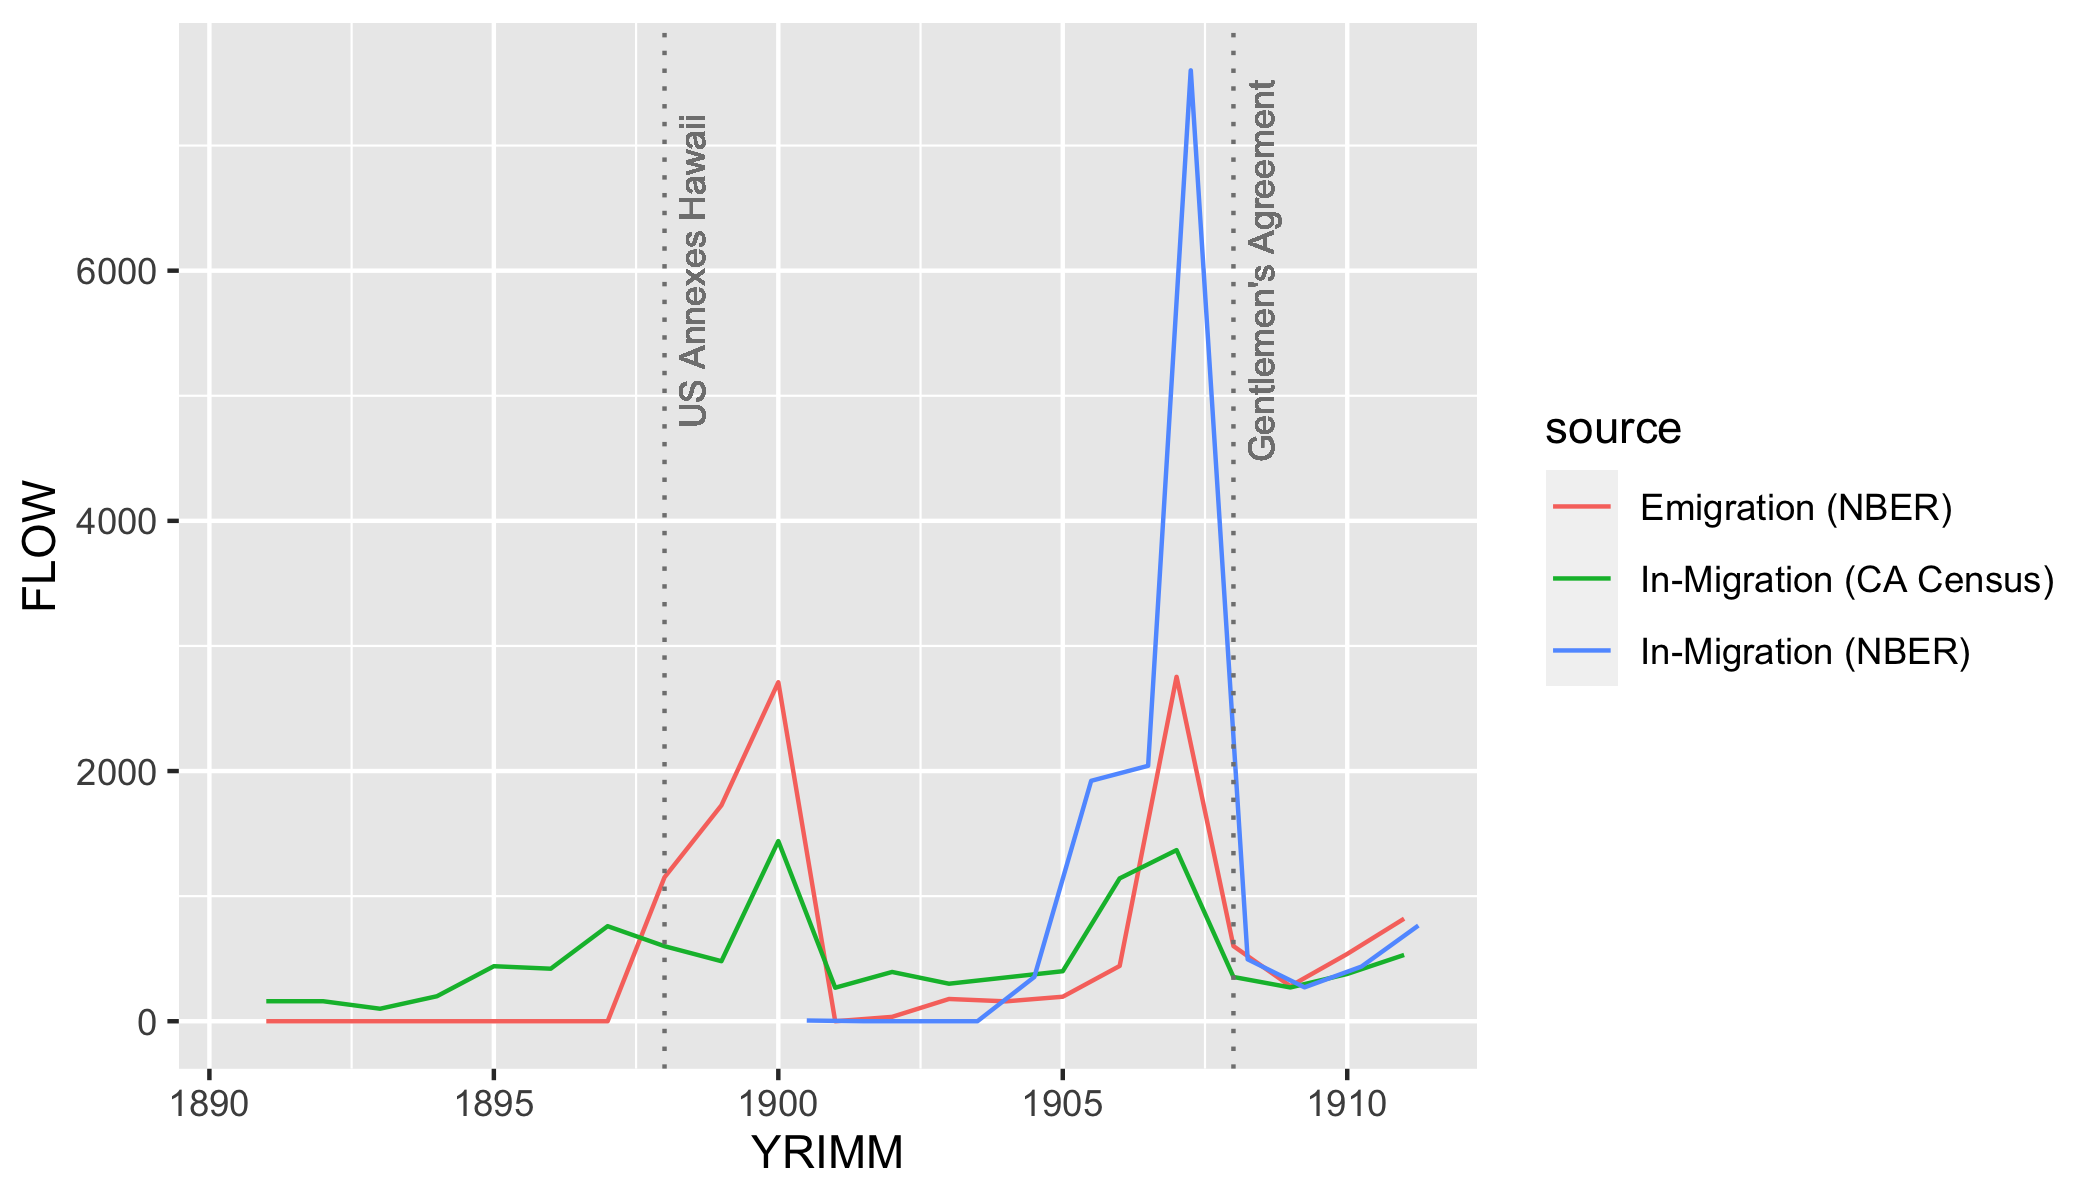
\includegraphics[width = \textwidth]{../../figs/6sep23/japan_flow.png}
    \end{figure}
\end{frame}

\begin{frame}
    \frametitle{Explaining Spikes in Japanese Immigration}
    \begin{itemize}
        \item 1906-07 spike easier -- anticipation of 1908 Gentlemen's Agreement
        \item 1900 spike less clear -- also shows up in emigration to US and in total emigration (mostly to Hawaii) but one year earlier in 1899. Possibily due to 1898 annexation of Hawaii and resulting instability -- temporary substitution towards US/CA? 
        \hyperlink{japan_emig}{\beamerbutton{All Japanese Emigration}}
    \end{itemize}
\end{frame}

% PART 1: IMMIGRATION INFLOW EFFECTS
\section{Immigration Inflow}
\begin{frame}[label = flow_reg]
    \frametitle{Immigration Inflow: Regression Specification}
    Old Equation:
    \begin{multline}
        \text{FLOW}_t = \alpha + \beta_1\text{TOTALIMM}_t + \beta_2\text{GNPGROWTH}_t +  \\ \textcolor{red}{\delta_1 t + \delta_2 t^2} + \sum_{\tau \in \mathcal{T}} \gamma^{FLOW}_\tau \mathbf{1}[TAX_t = \tau] 
    \end{multline}
    New Equation V1 (adding sending country population stock):
    \begin{multline}
        \text{FLOW}_t = \alpha + \beta_1\text{TOTALIMM}_t + \beta_2\text{GNPGROWTH}_t +  \\ \textcolor{blue}{\beta_3 POPSTOCK_t} + \sum_{\tau \in \mathcal{T}} \gamma^{FLOW}_\tau \mathbf{1}[TAX_t = \tau] 
    \end{multline}
\end{frame}

\begin{frame}[label = flow_graph]
    \frametitle{Graphing $\gamma_\tau^{FLOW}$'s for Various Countries [Eq (2)]}
    \centering
    \begin{figure}
        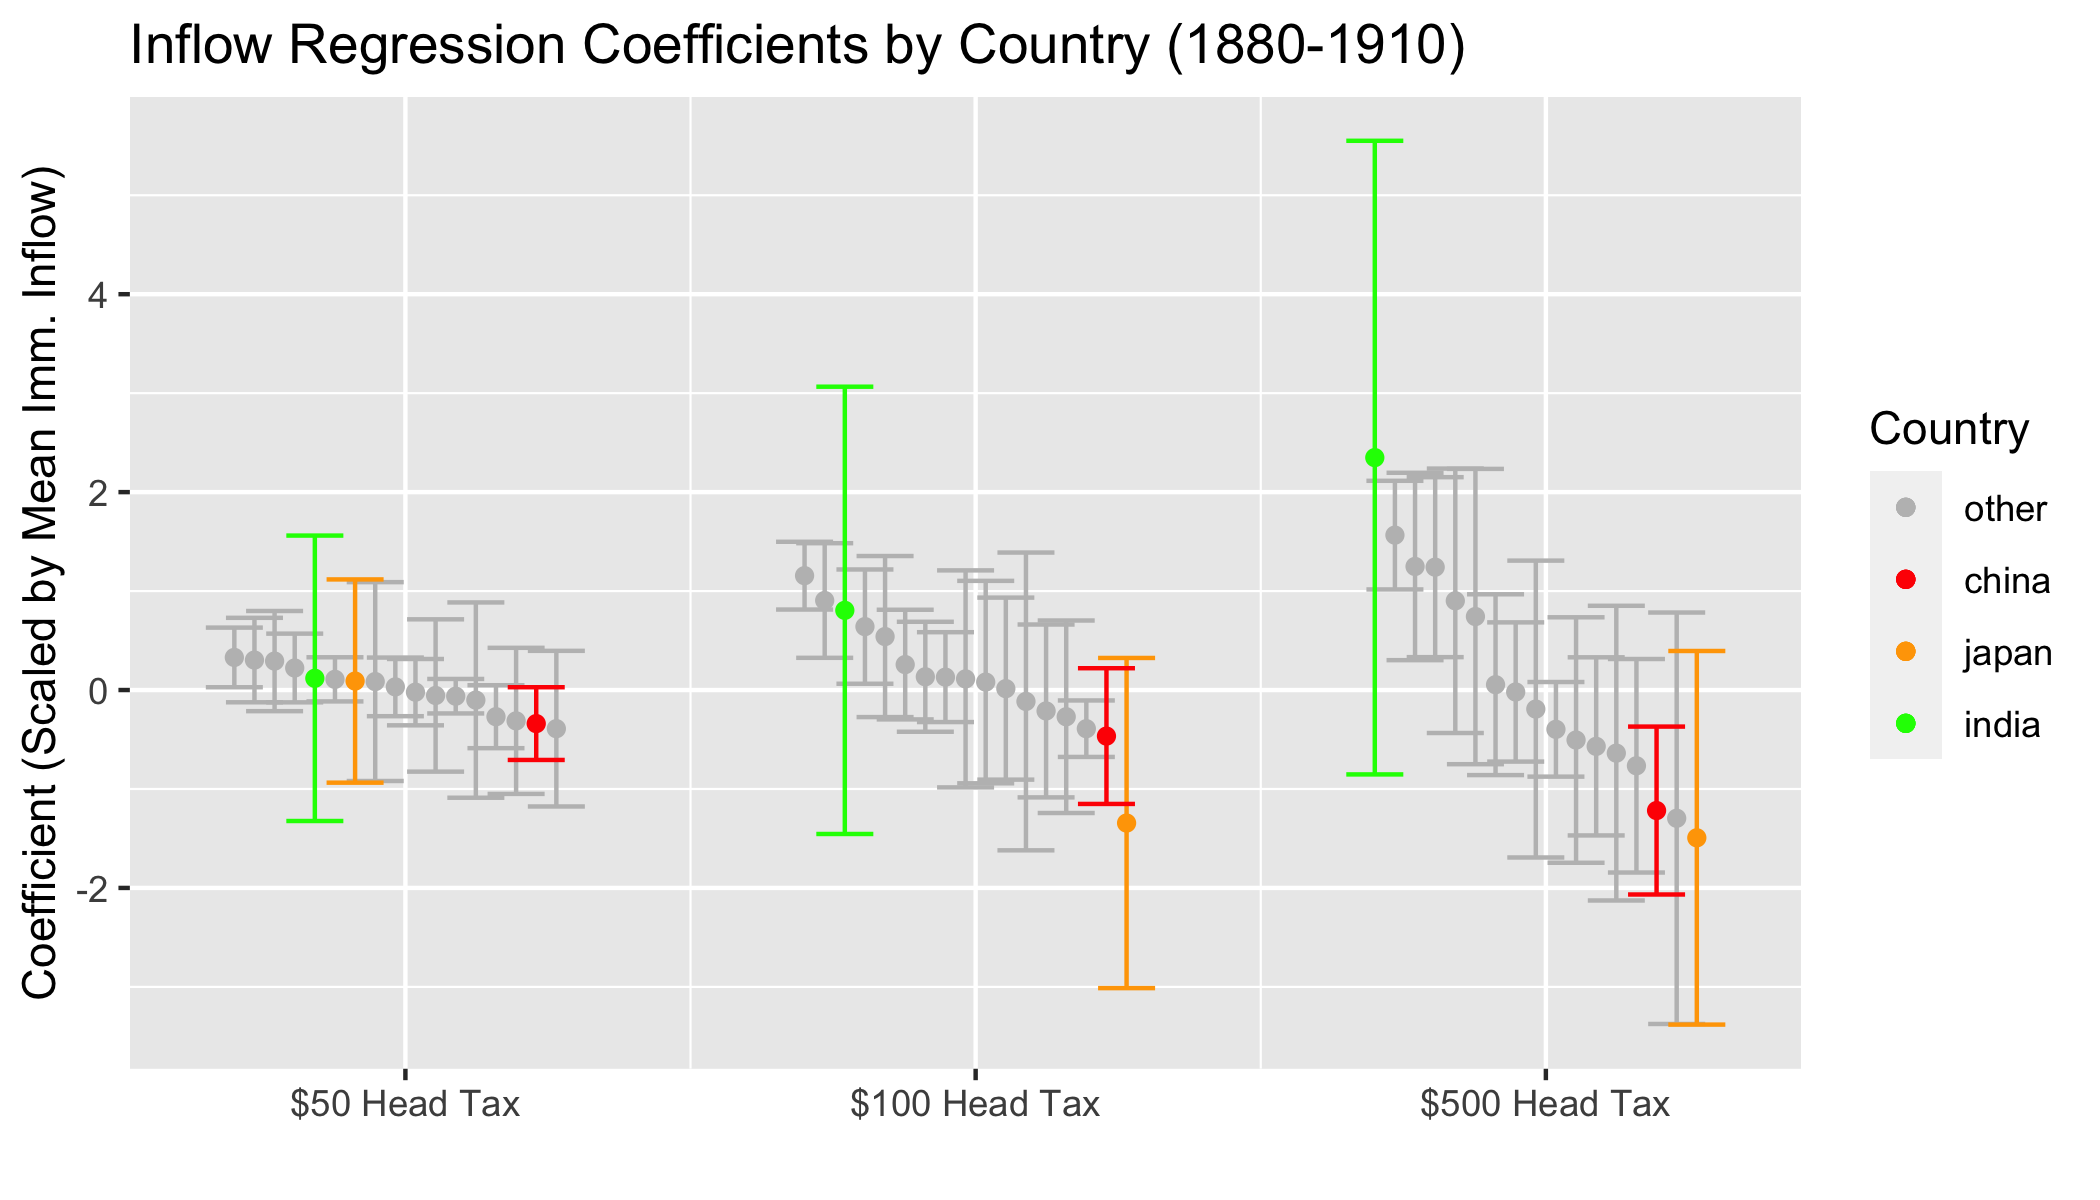
\includegraphics[width = \textwidth]{../../figs/6sep23/reg_coefs.png}
    \end{figure}
    \hyperlink{flow_graph_old}{\beamerbutton{Old Version}}
\end{frame}

\begin{frame}[label = flow_reg2]
    \frametitle{Immigration Inflow: Regression Specification 2}
    New Equation V2 (adding dummies for first two years of new tax):
    \begin{multline}
        \text{FLOW}_t = \alpha + \beta_1\text{TOTALIMM}_t + \beta_2\text{GNPGROWTH}_t +  \beta_3 POPSTOCK_t + \\ \sum_{\tau \in \mathcal{T}} \Big\{ \gamma^{FLOW}_\tau \mathbf{1}[TAX_t = \tau] + \textcolor{blue}{\phi^{FLOW}_\tau \mathbf{1}[TAX_t = \tau] \mathbf{1}[t - YEAR_{\tau} \leq 2]} \Big\}
    \end{multline}
    where $YEAR_{\tau}$ represents the first year where the tax was equal to $\tau$. $\phi^{FLOW}_\tau$ represents \textbf{additional} effect of the head tax in the two years following a change.

    Doesn't seem to make much of a difference for these regressions (data cut too thinly).
\end{frame}

% \begin{frame}[label = flow_graph]
%     \frametitle{Graphing $\phi_\tau^{FLOW}$'s for Various Countries [Eq (2)]}
%     \centering
%     \begin{figure}
%         \includegraphics[width = \textwidth]{../../figs/6sep23/reg_coefs2.png}
%     \end{figure}
%     \hyperlink{flow_graph_old}{\beamerbutton{Old Version}}
% \end{frame}

%%%%%%%%%%%%%%%%%%%%%%%%%%%%%%%%%%%%%%%%%%%%%%%%%%%%%%%
%%%%%%%%%%      A  P  P  E  N  D  I  X      %%%%%%%%%%%
%%%%%%%%%%%%%%%%%%%%%%%%%%%%%%%%%%%%%%%%%%%%%%%%%%%%%%%
\appendix 

\begin{frame}[label = japan_emig]
	\frametitle{Emigration from Japan}
    \centering
	\begin{figure}[H]
		\begin{center}
			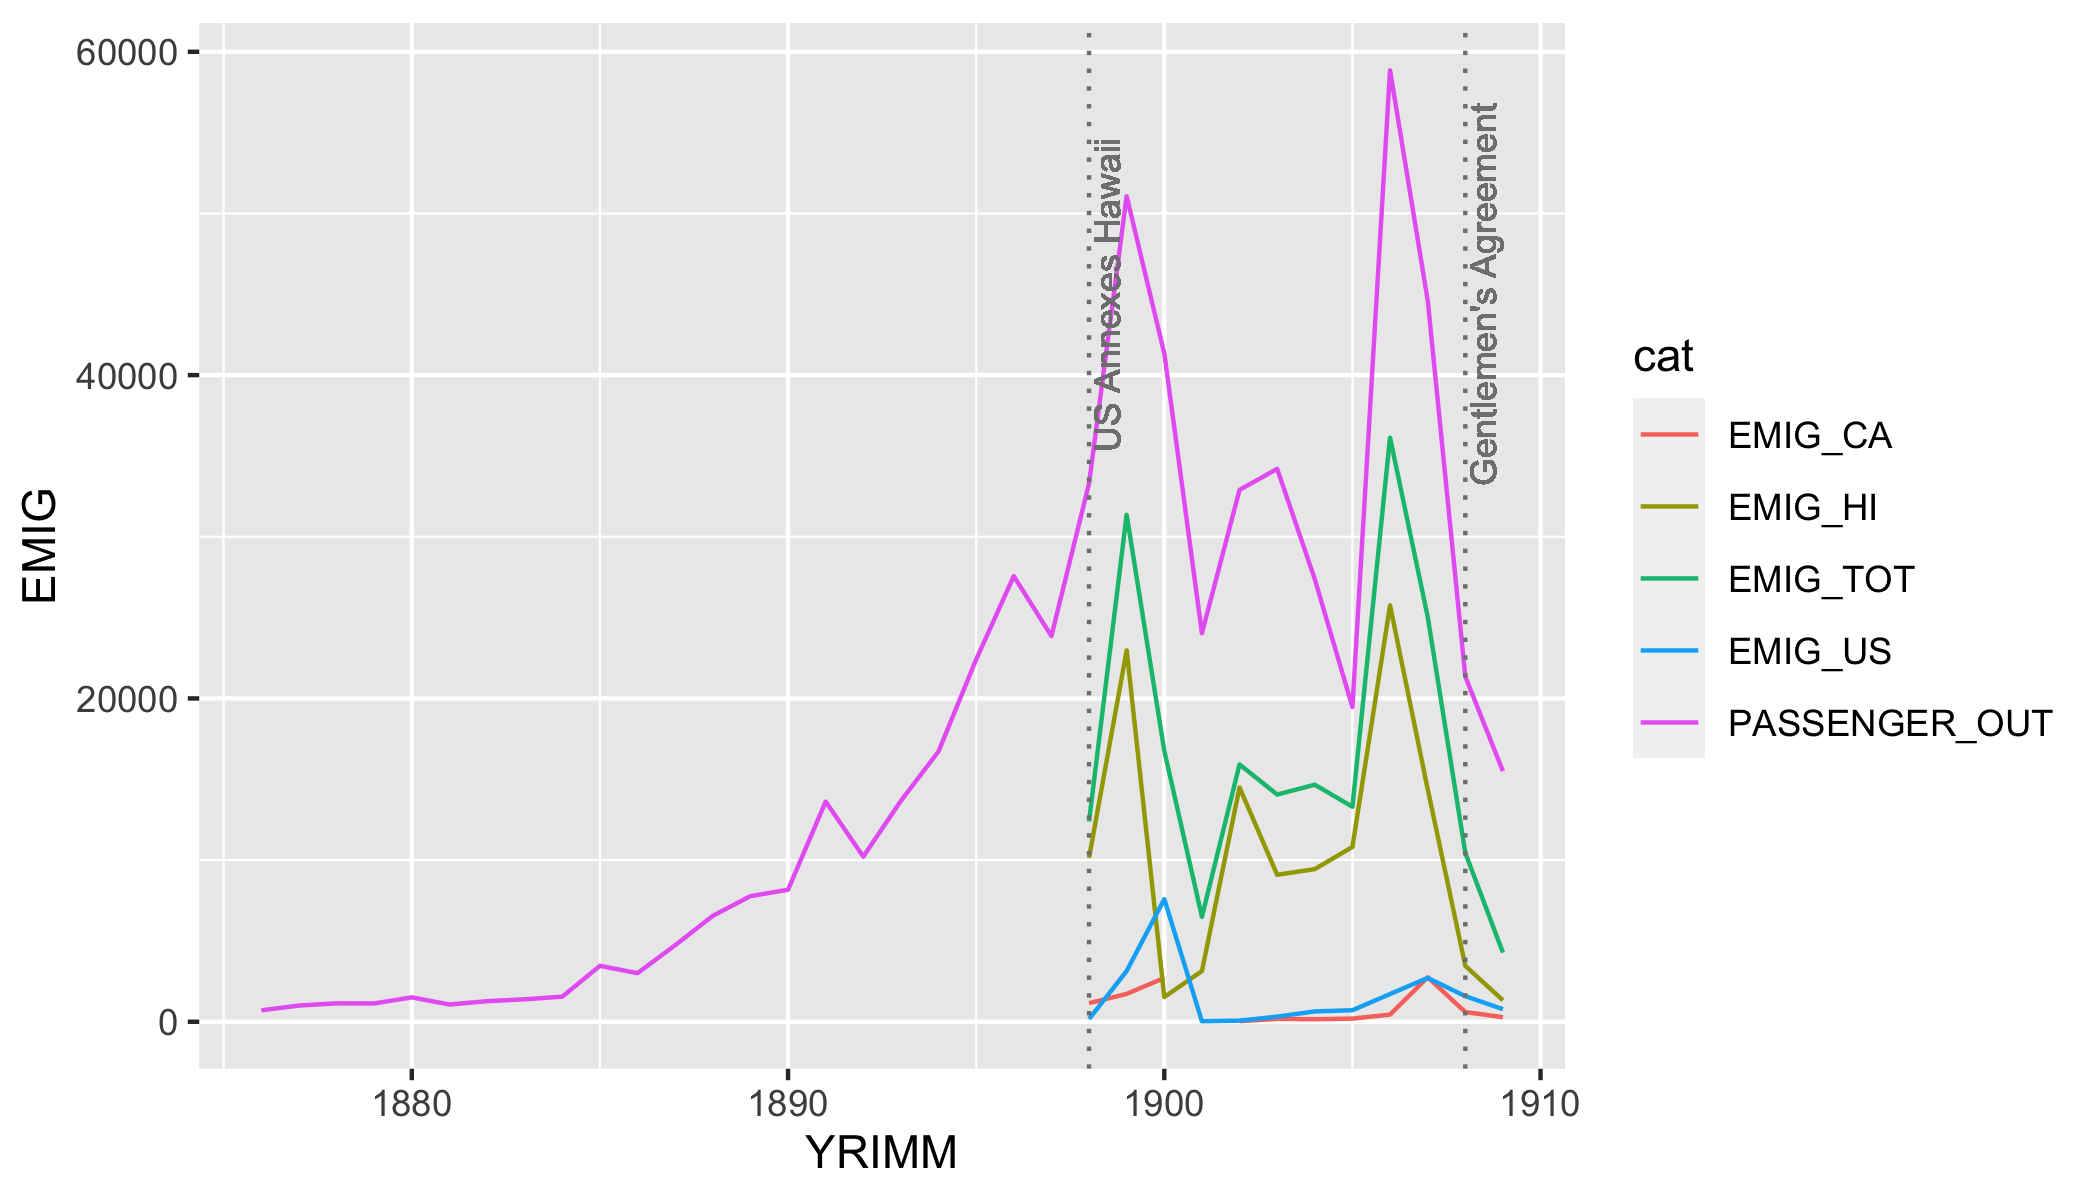
\includegraphics[width=\textwidth]{../../figs/6sep23/japan_emig.png}
		\end{center}
	\end{figure}
    \hyperlink{japanflow}{\beamerbutton{Back to Slides}}
\end{frame}

\begin{frame}[label = hk_departure]
	\frametitle{1895 HK Emigration Records}
    \centering
	\begin{figure}[H]
		\begin{center}
			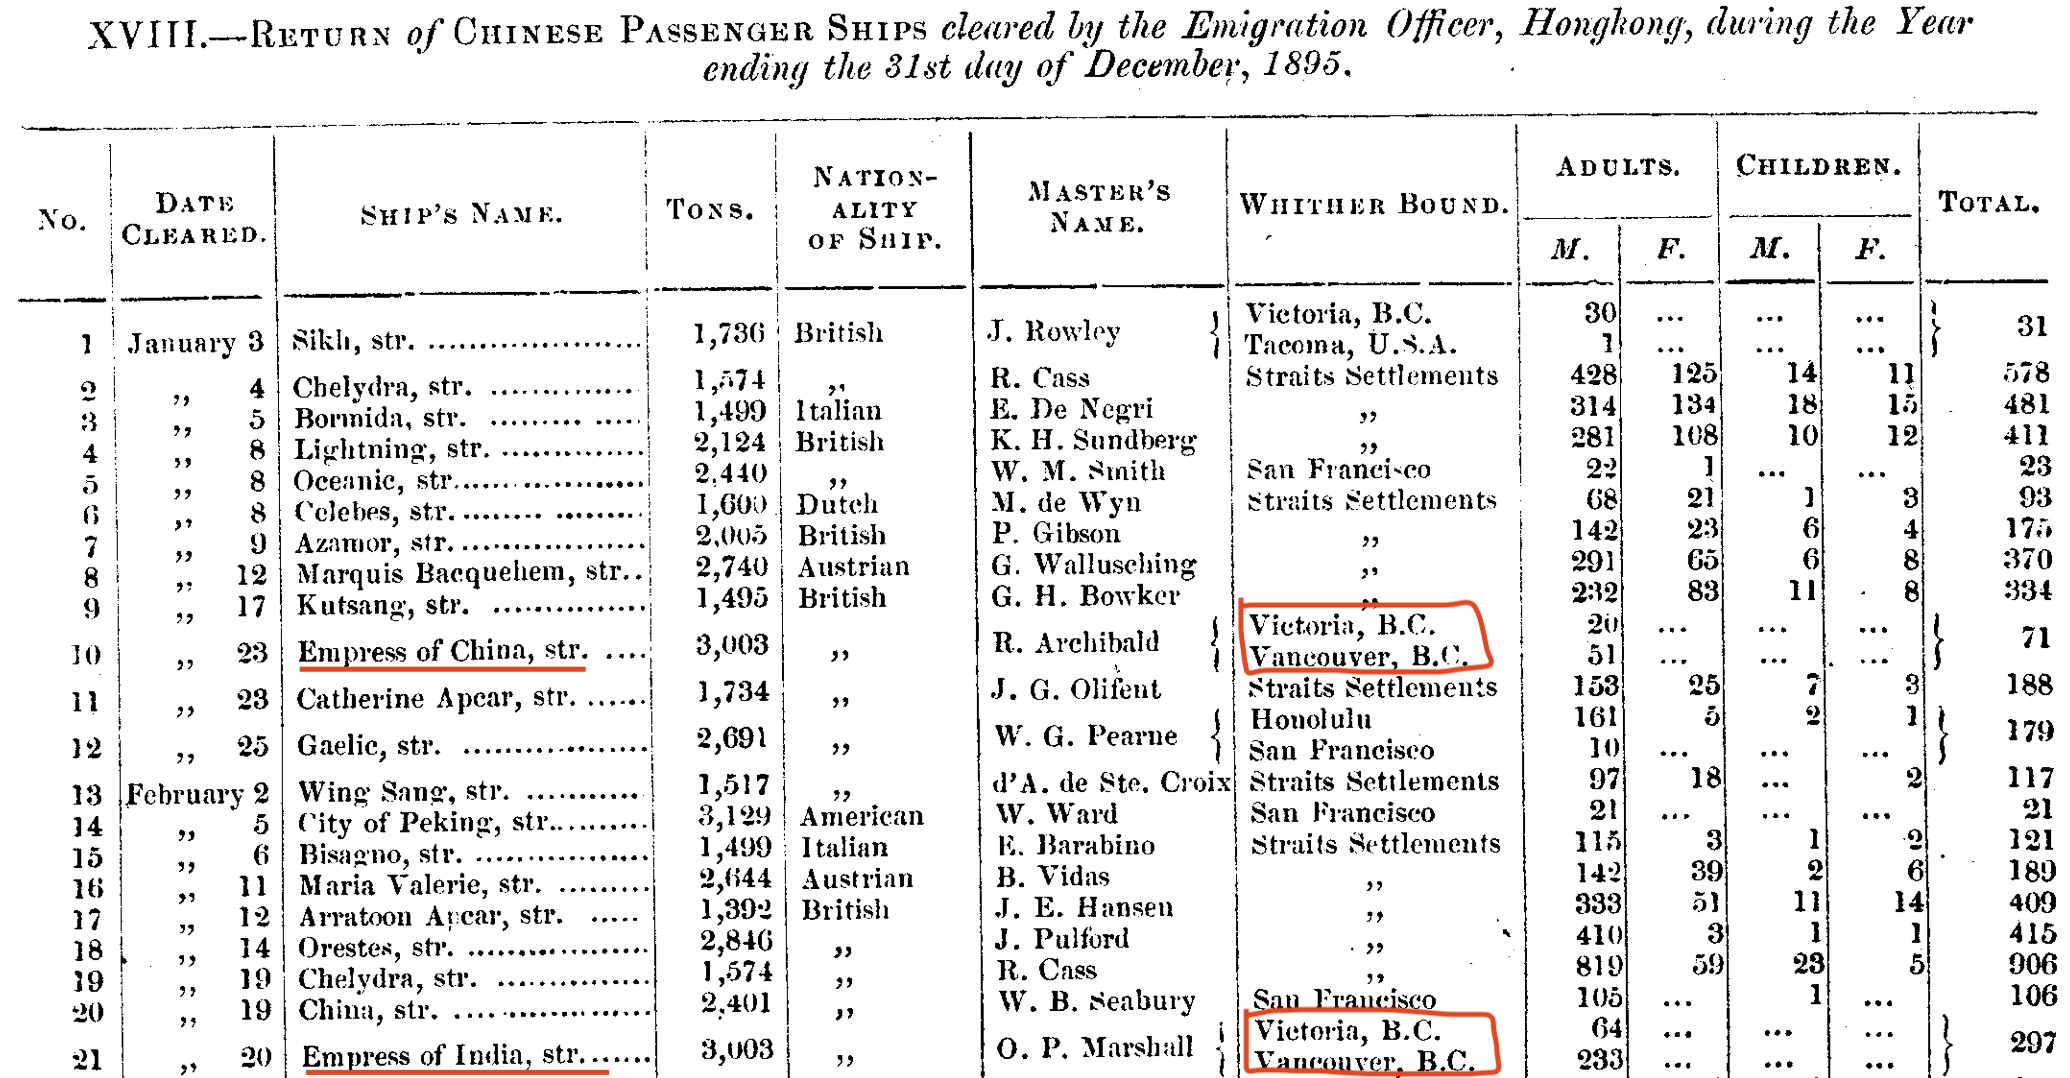
\includegraphics[width=\textwidth]{../../figs/6sep23/hk_departure_1895.jpg}
		\end{center}
	\end{figure}
    \hyperlink{departure}{\beamerbutton{Back to Slides}}
\end{frame}

\begin{frame}[label = reg_summ]
	\frametitle{1895 CA Chinese Register Summary by Conveyance}
    \centering
	\begin{figure}[H]
		\begin{center}
			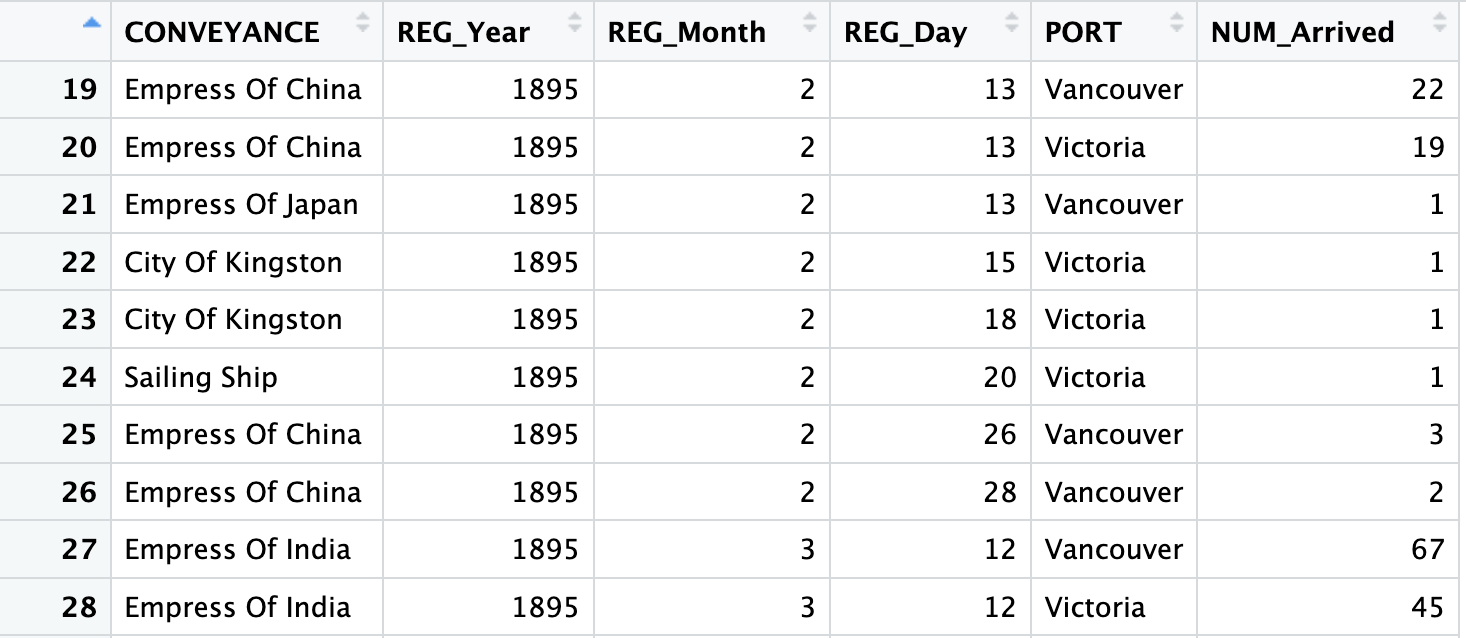
\includegraphics[width=\textwidth]{../../figs/6sep23/register_summ_1895.png}
		\end{center}
	\end{figure}
    \hyperlink{departure}{\beamerbutton{Back to Slides}}
\end{frame}

\begin{frame}[label = hk_return]
	\frametitle{1895 HK Immigration Records}
    \centering
	\begin{figure}[H]
		\begin{center}
			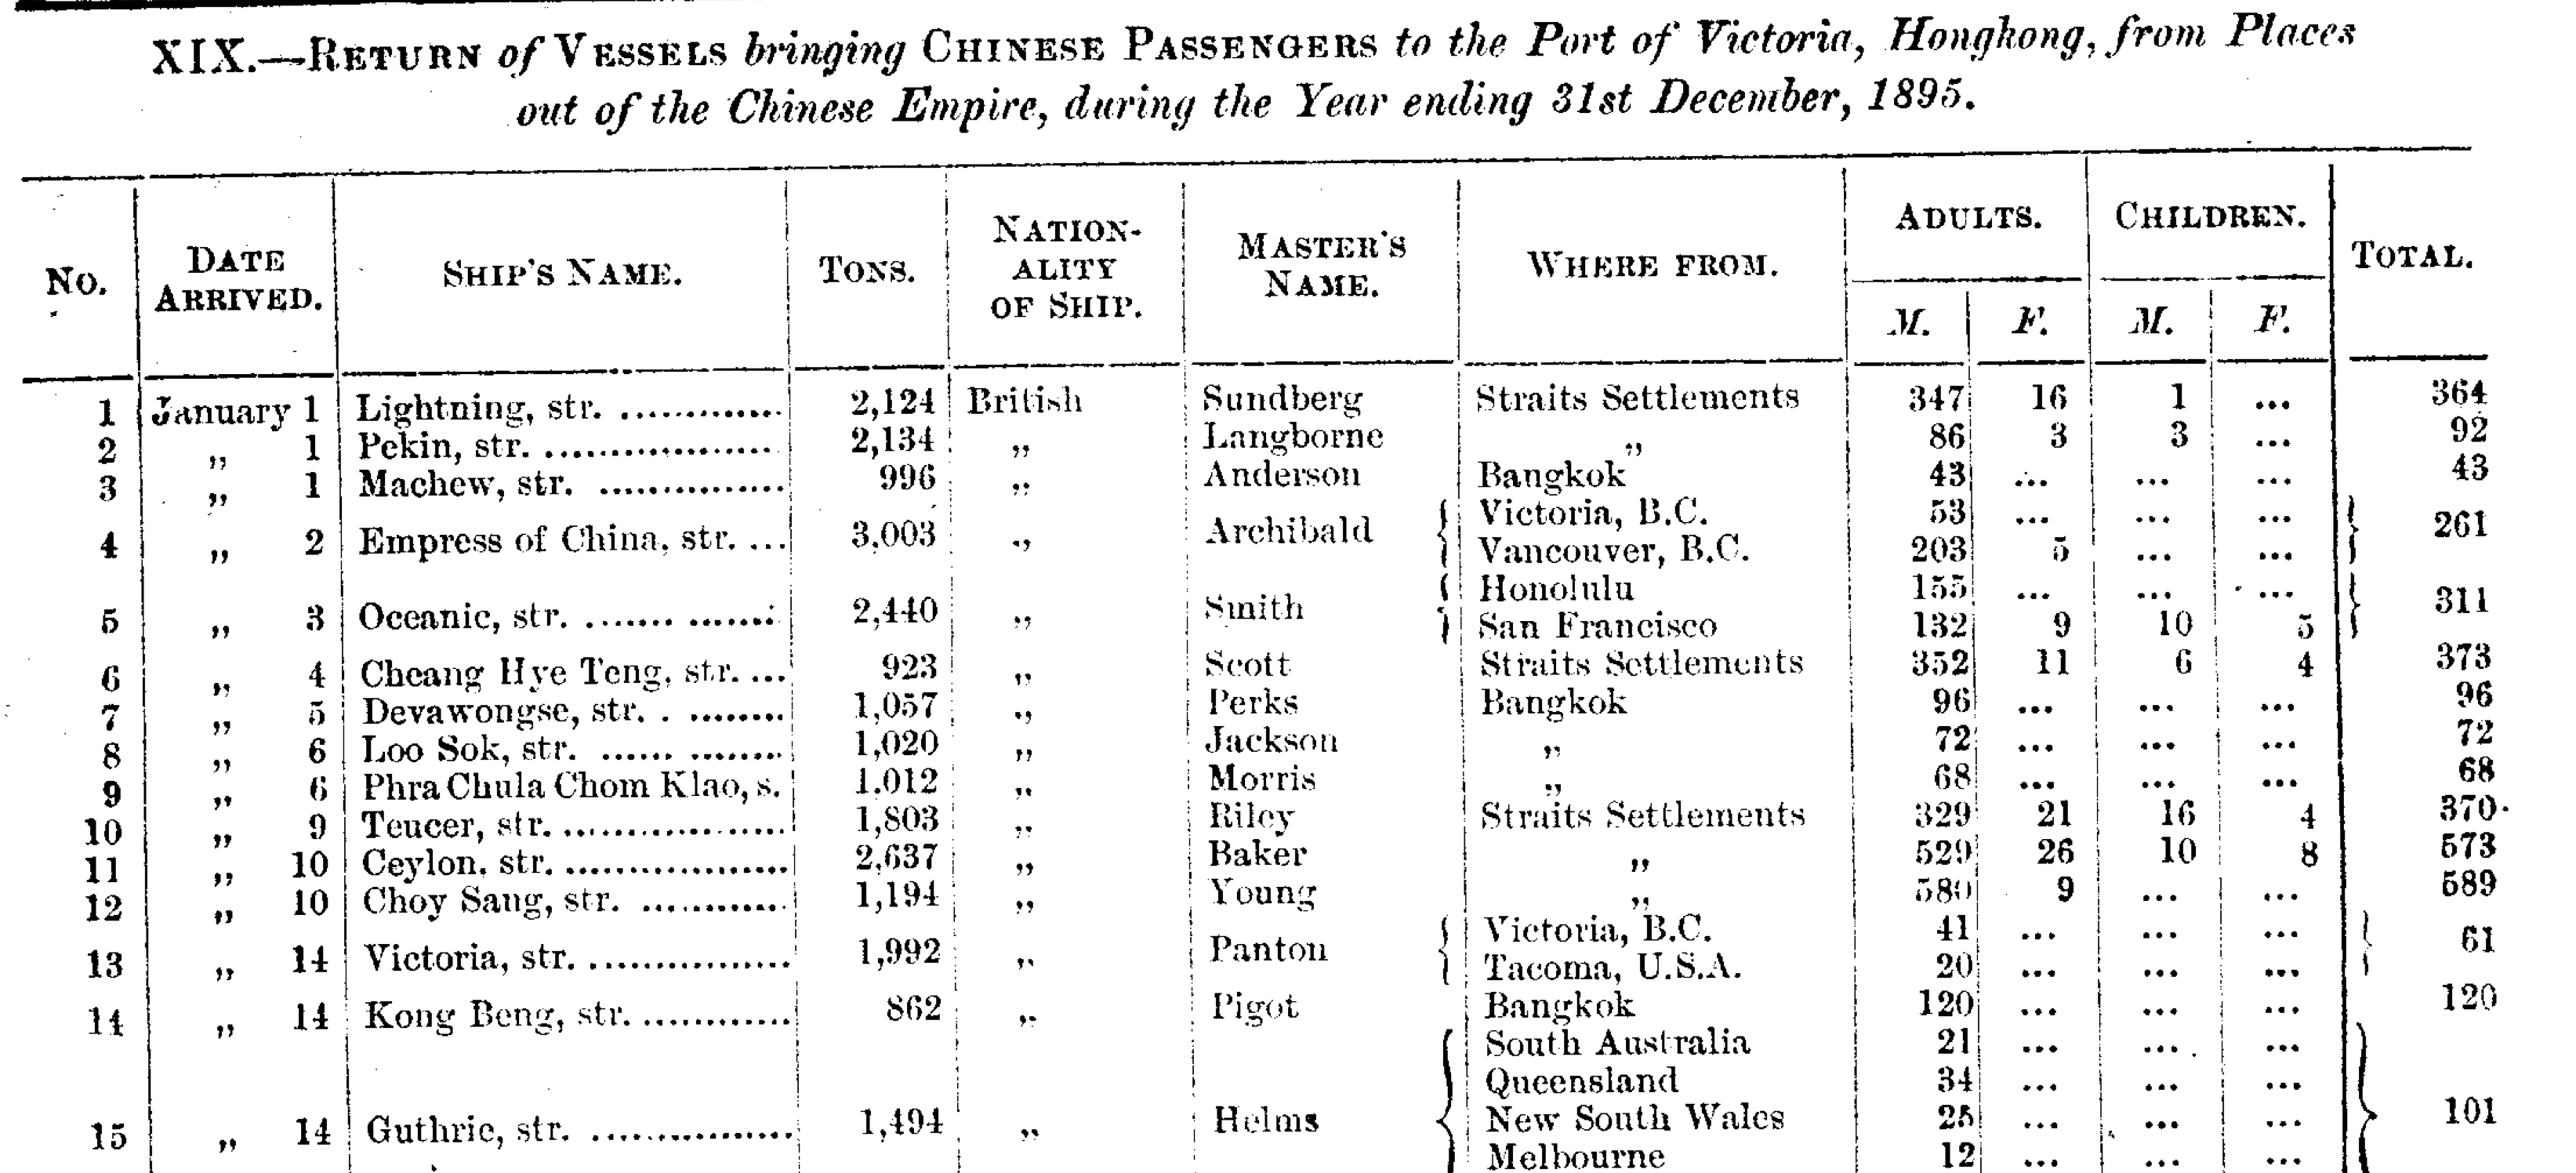
\includegraphics[width=\textwidth]{../../figs/6sep23/hk_return_1895.png}
		\end{center}
	\end{figure}
    \hyperlink{departure}{\beamerbutton{Back to Slides}}
\end{frame}

\begin{frame}[label = china_emig_mckeown]
    \frametitle{Emigration from South China (McKeown 2010)}
    \centering
    \begin{figure}
        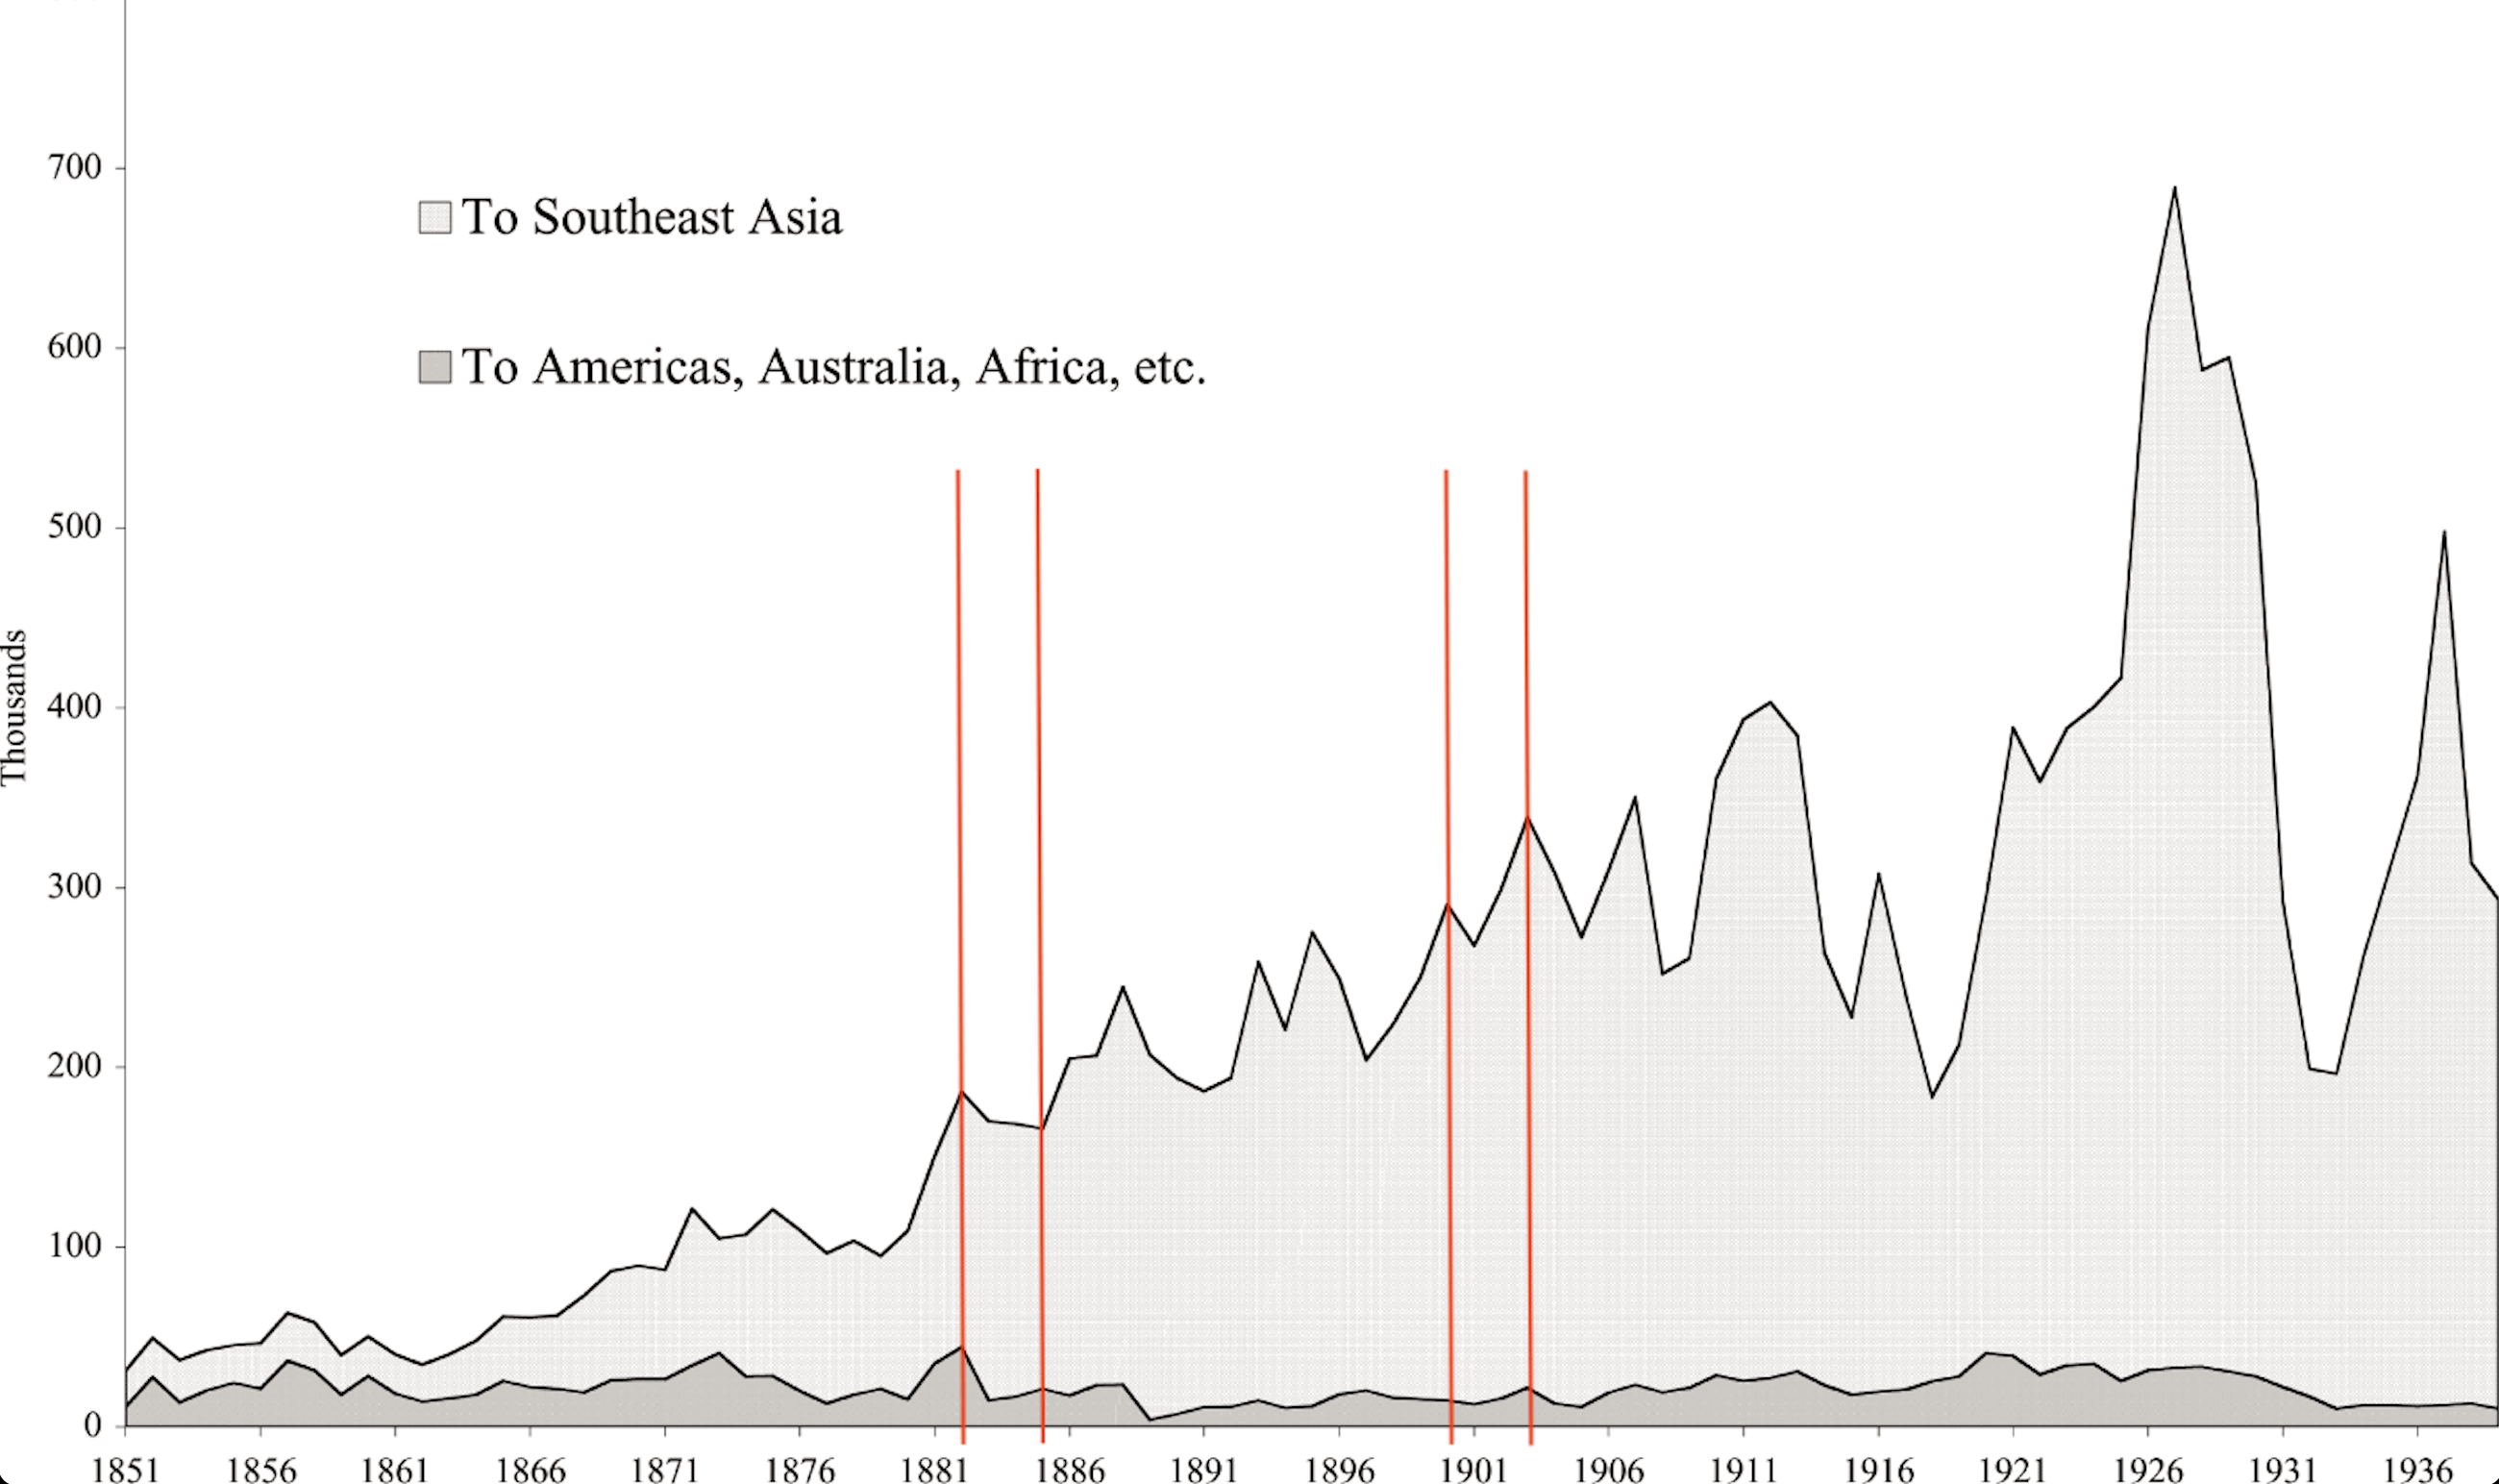
\includegraphics[width = \textwidth]{../../figs/6sep23/china_emig_mckeown.png}
    \end{figure}
    \hyperlink{chinaflow}{\beamerbutton{Back to Slides}}
\end{frame}


\begin{frame}[label = flow_graph_old]
    \frametitle{Graphing $\gamma_\tau^{FLOW}$'s for Various Countries Old Version [Eq (1)]}
    \centering
    \begin{figure}
        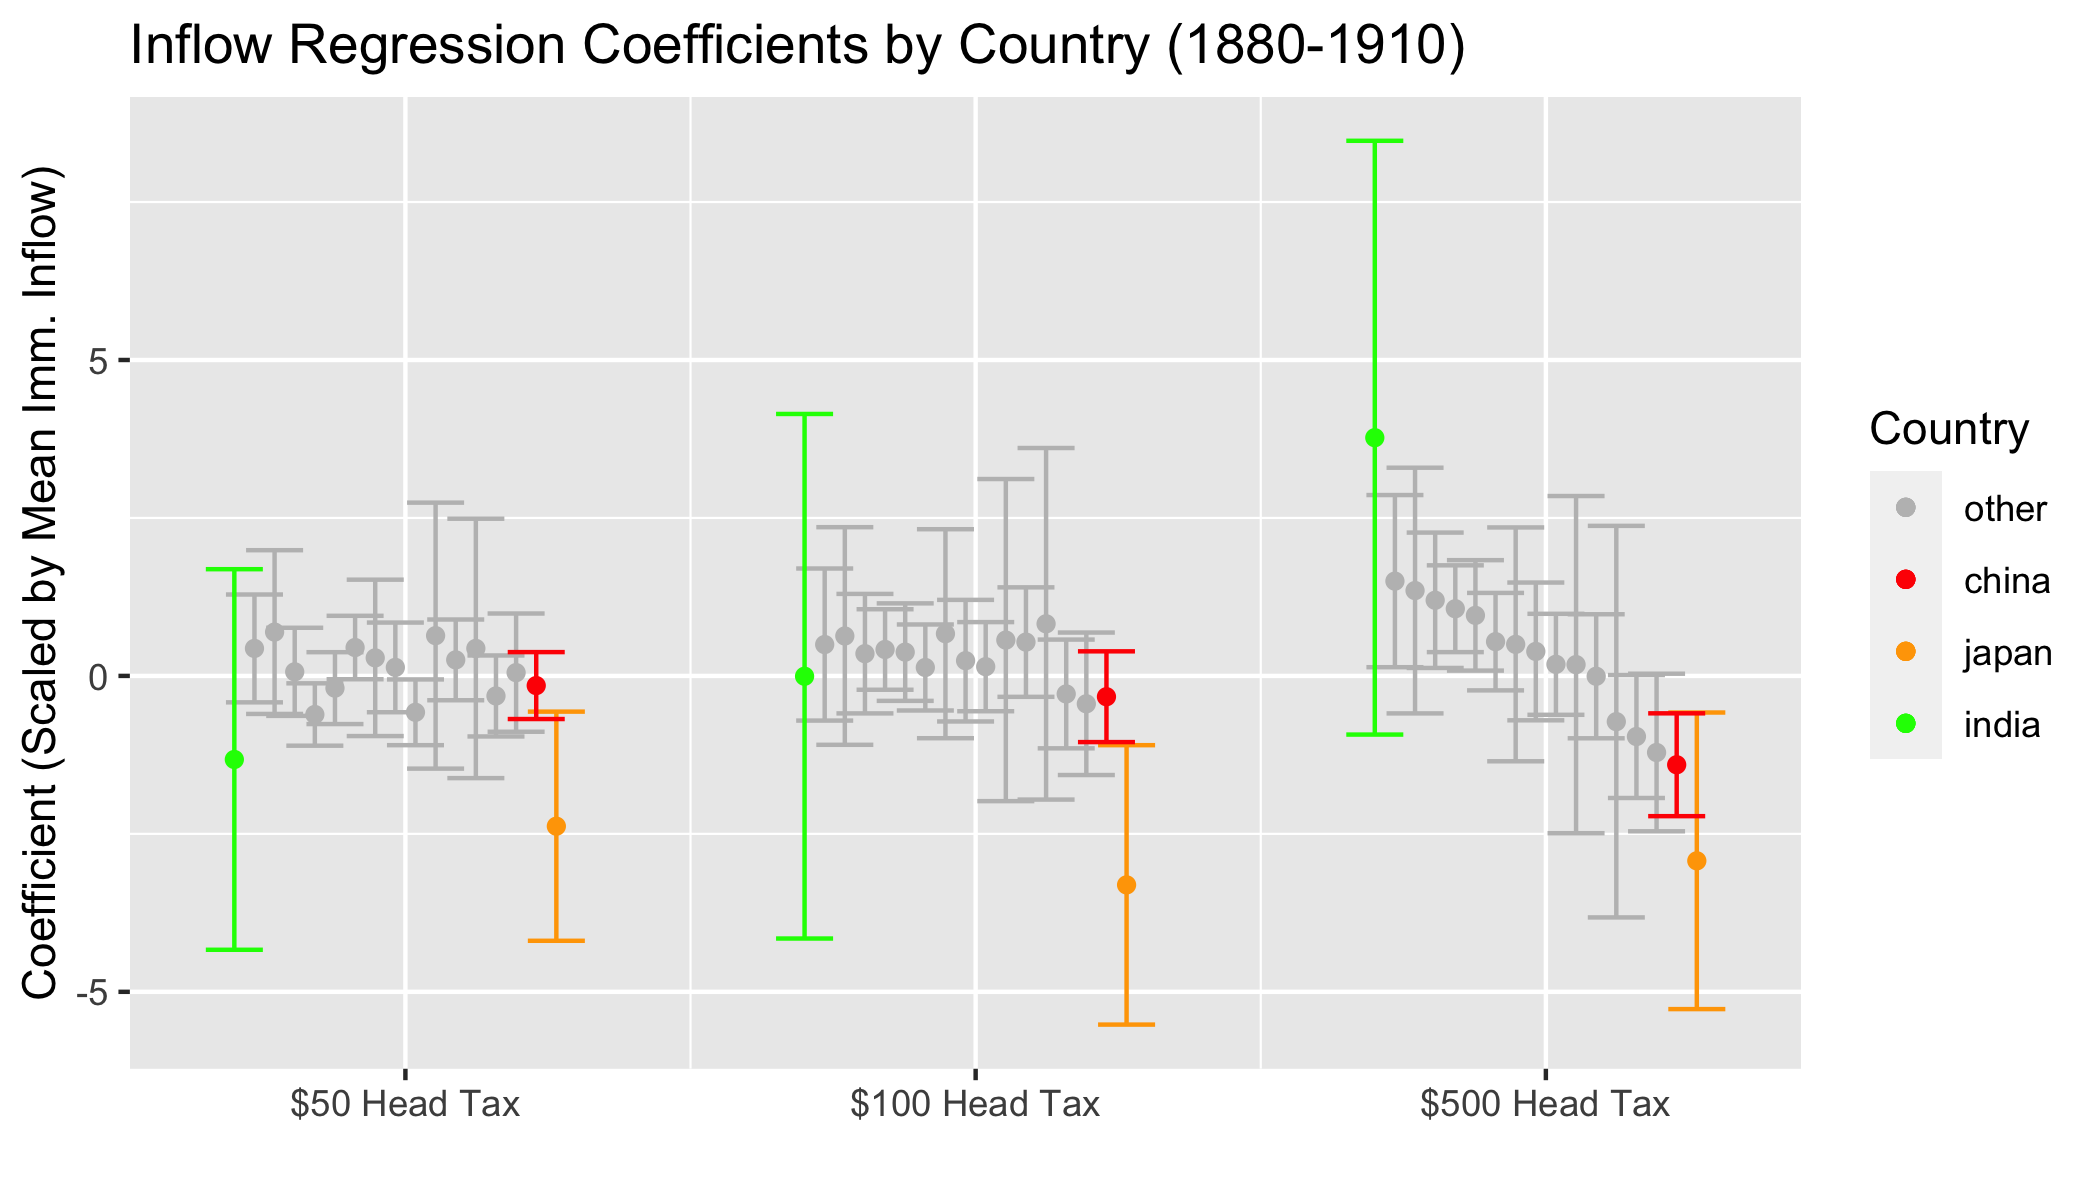
\includegraphics[width = \textwidth]{../../figs/8aug23/reg_coefs.png}
    \end{figure}
    \hyperlink{flow_graph}{\beamerbutton{Back to Slides}}
\end{frame}

\end{document}